% Exam Template for UMTYMP and Math Department courses
%
% Using Philip Hirschhorn's exam.cls: http://www-math.mit.edu/~psh/#ExamCls
%
% run pdflatex on a finished exam at least three times to do the grading table on front page.
%
%%%%%%%%%%%%%%%%%%%%%%%%%%%%%%%%%%%%%%%%%%%%%%%%%%%%%%%%%%%%%%%%%%%%%%%%%%%%%%%%%%%%%%%%%%%%%%

% These lines can probably stay unchanged, although you can remove the last
% two packages if you're not making pictures with tikz.
\documentclass[11pt]{exam}
\RequirePackage{amssymb, amsfonts, amsmath, mathtools, latexsym, verbatim, xspace, setspace}
\RequirePackage{tikz, pgflibraryplotmarks}

% By default LaTeX uses large margins.  This doesn't work well on exams; problems
% end up in the "middle" of the page, reducing the amount of space for students
% to work on them.
\usepackage[margin=1in]{geometry}


% Here's where you edit the Class, Exam, Date, etc.
\newcommand{\class}{Math 1271 - Lectures 010 and 030 }
\newcommand{\term}{Fall 2017}
\newcommand{\examnum}{Quiz 6A}
\newcommand{\examdate}{10/20/17}
\newcommand{\timelimit}{25 Minutes}
\DeclarePairedDelimiter\abs{\lvert}{\rvert}%
% For an exam, single spacing is most appropriate
\singlespacing
% \onehalfspacing
% \doublespacing

% For an exam, we generally want to turn off paragraph indentation
\parindent 0ex
\def\changemargin#1#2{\list{}{\rightmargin#2\leftmargin#1}\item[]}
\let\endchangemargin=\endlist 
\usepackage{enumitem}
\renewcommand{\d}{\mathrm{d}}
\begin{document} 

% These commands set up the running header on the top of the exam pages
\pagestyle{head}
\firstpageheader{}{}{}
\runningheader{\class}{\examnum\ - Page \thepage\ of \numpages}{\examdate}
\runningheadrule

\begin{flushright}
\begin{tabular}{p{2.8in} r l}
\textbf{\class} & \textbf{Name (Print):} &\makebox[2in]{\hrule David DeMark}\\
\textbf{\term} &&\\
\textbf{\examnum} &&\\
\textbf{\examdate} &&\\
\textbf{Time Limit: \timelimit} & Section & \makebox[2in]{\hrule 012 \& 016}
\end{tabular}\\
\end{flushright}
\rule[1ex]{\textwidth}{.1pt}

You may \textit{not} use your books, notes, graphing calculator, phones or any other internet devices on this exam.\\

You are \textbf{required} to show your work on each problem on this quiz.\\
\hspace*{12cm}\begin{minipage}[t]{2.3in}
\vspace{0pt}
%\cellwidth{3em}
\gradetablestretch{2}
\vqword{Problem}
\addpoints % required here by exam.cls, even though questions haven't started yet.	
\gradetable[v]%[pages]  % Use [pages] to have grading table by page instead of question

\end{minipage}
%\newpage % End of cover page

%%%%%%%%%%%%%%%%%%%%%%%%%%%%%%%%%%%%%%%%%%%%%%%%%%%%%%%%%%%%%%%%%%%%%%%%%%%%%%%%%%%%%
%
% See http://www-math.mit.edu/~psh/#ExamCls for full documentation, but the questions
% below give an idea of how to write questions [with parts] and have the points
% tracked automatically on the cover page.
%
%
%%%%%%%%%%%%%%%%%%%%%%%%%%%%%%%%%%%%%%%%%%%%%%%%%%%%%%%%%%%%%%%%%%%%%%%%%%%%%%%%%%%%%


\begin{questions}

% Basic question
%\vspace*{-130pt}
\addpoints\question[3] Find the absolute minimum and absolute maximum on the given interval $$x^3-65x+10,\:\:\:[-5,6]$$
\vspace{3em}\indent Two steps here. 1) Identify critical points and 2) plug those and our endpoints into the function (which I'll call $f$).

1) $f'(x)=3x^2-75$. $f'(x)=0$ for $x=\pm 5$. $f'$ exists everywhere.

2) $f(-5)=260$, $f(5)=-240$, $f(6)=-224$. Thus, we have an absolute minimum at $(5,-240)$ and absolute maximum at $(-5,260)$.
% Question with parts
\newpage
\addpoints
\question With the given function $$y=\sqrt{13-x^2}$$\begin{parts}
	\part[2] Find the differential $\mathrm d y$.
	\part[1] Evaluate $\mathrm d y$ for $x=2$ and $\mathrm d x=.1$.
\end{parts}\vskip10mm
\begin{enumerate}[label=(\alph*)]
	\item We have that for $y=f(x)$, $\d y=\d f(x)=f'(x)\d x$. Thus, $$\d y=\d(\sqrt{13-x^2})=\frac{-x\d x}{\sqrt{13-x^2}}$$
	\item Substitute in $x=2$, $\d x=.1$ to the line above.
	$$\d y=\frac{-(2)(.1)}{\sqrt{13-(2)^2}}=\frac{-1}{15}$$
\end{enumerate}
\vskip15mm
\addpoints
\question[4] A ladder 12 m long rests against a vertical wall. If the bottom of the ladder slides away from the wall at a rate of 2 m/s, how fast is the top of the ladder sliding down the wall when the bottom of the ladder is 5 m away from the wall?
%\addpoints
Our set-up is as follows: We draw a triangle with vertices at the ladder's resting place on the wall, the corner between the floor and the wall, and the ladder's resting place on the floor.
Let's draw a picture and label some stuff
\begin{figure}[h!]\centering
	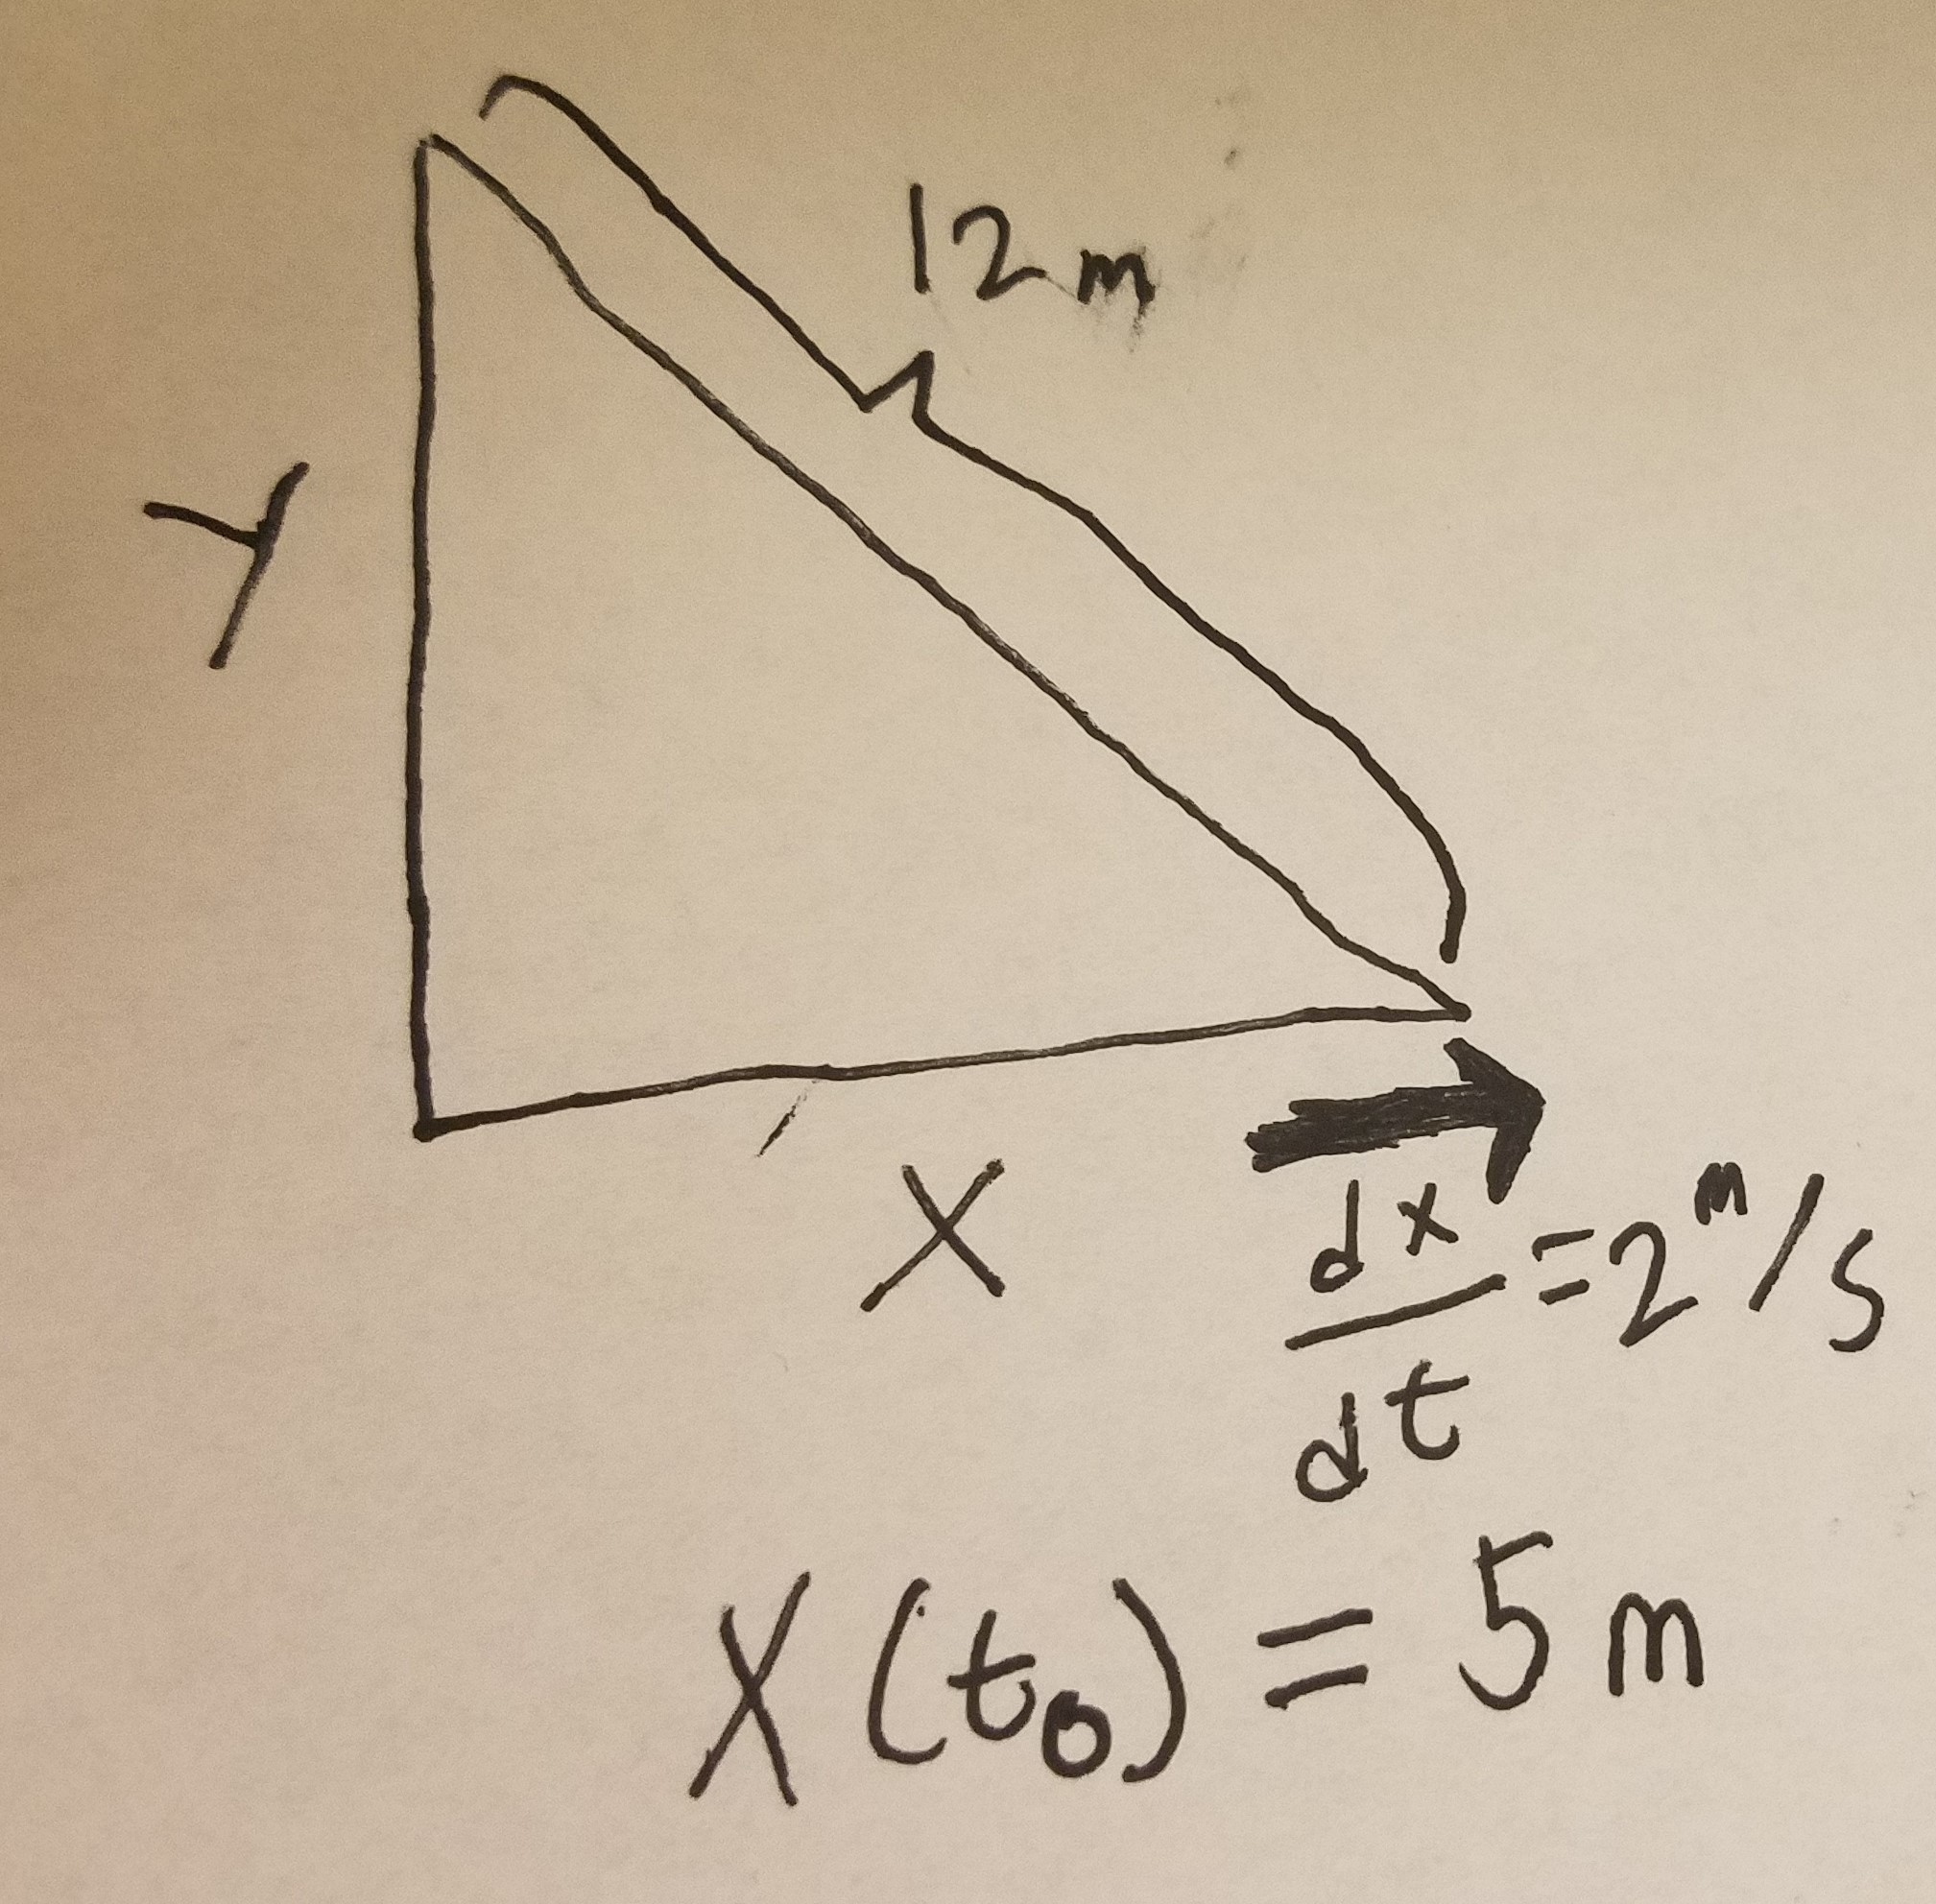
\includegraphics[scale=.1]{q6p3}\caption{A triangle, labeled with the relevant data from the problem.}
\end{figure} 

\textbf{Known:} $x(t_0)=5$m, $\frac{\d x}{\d t}=2$m/s, $x^2+y^2=12^2.$ \textbf{Unknown}: $y'(t_0)$.

We can relate $y'$ and $x'$ by differentiating: \begin{align*}
x(t)^2+y(t)^2&=12^2\\\frac{\d}{\d t}\left(x(t)^2+y(t)^2\right)&=\frac{\d}{\d t}\left(12^2\right)\\
2x(t)*x'(t)+2y(t)*y'(t)&=0\\
\implies y'(t)=\frac{-x(t)*x'(t)}{y(t)}
\end{align*}
To find $y'(t_0)$, we need $x(t_0)$ (which we have already), $x'(t_0)$ (ditto) and $y(t_0)$. But $12^2=x(t_0)^2+y(t_0)^2=25+y(t_0)^2\implies y(t_0)=\sqrt{144-25}=\sqrt{119}$. Now, $$y'(t_0)=\frac{-x(t_0)x'(t_0)}{y(t_0)}=\frac{-(5)(2)}{\sqrt{119}}=\frac{-10}{\sqrt{119}}$$


\question (Bonus 2 points) Write the definition of a critical number.

Relative to a function $f$, a critical number $c$ is one at which $f'(c)=0$ or $f'(c)$ does not exist

(note: this is all that is needed\textemdash anything about maxima or minima or endpoints is superfluous.)
\end{questions}
\end{document}